\documentclass[border=1mm]{standalone}

\usepackage[dvipsnames]{xcolor}
\usepackage{hyperref}

\colorlet{myblue}{RoyalBlue}
\colorlet{myred}{WildStrawberry}
\colorlet{myorange}{Melon}
\colorlet{mygreen}{OliveGreen}
\colorlet{myviolet}{RoyalPurple}
\colorlet{myyellow}{Goldenrod}
\hypersetup{urlbordercolor=Green, linkbordercolor=Blue}

\usepackage[dvipsnames]{xcolor}
\usepackage{tikz}
\usetikzlibrary{positioning}

\begin{document}
	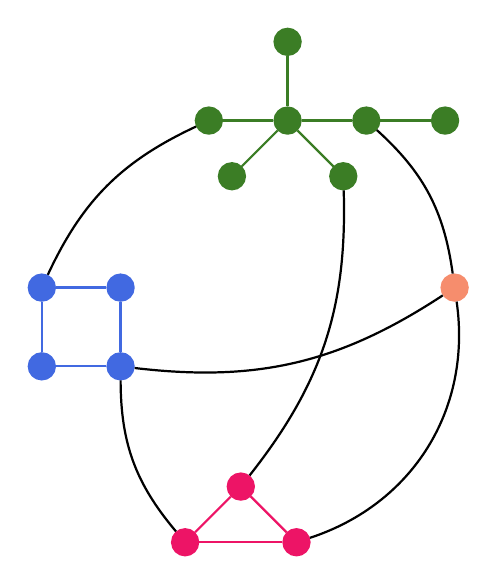
\begin{tikzpicture}[node distance={10mm}, thick, main/.style = {draw, circle, fill}]
		\node[main] (1) [color=mygreen] {};
		\node[main] (2) [above of=1] [color=mygreen] {};
		\node[main] (3) [below left of=1] [color=mygreen] {};
		\node[main] (4) [below right of=1] [color=mygreen] {};
		\node[main] (5) [left of=1] [color=mygreen] {};
		\node[main] (6) [right of=1] [color=mygreen] {};
		\node[main] (7) [right of=6] [color=mygreen] {};
		\node[main] (8) [below right of=6] [below right of=4] [color=myorange] {};
		\node[main] (9) [below left of=5] [below left of=3] [color=myblue] {};
		\node[main] (10) [left of=9] [color=myblue] {};
		\node[main] (11) [below of=10] [color=myblue] {};
		\node[main] (12) [below of=9] [color=myblue] {};
		\node[main] (13) [below right = 1.8cm of 12] [color=myred] {};
		\node[main] (14) [below left of=13] [color=myred] {};
		\node[main] (15) [below right of=13] [color=myred] {};
		\path[color=myblue] (9) edge (10)
			(9) edge (12)
			(10) edge (11)
			(11) edge (12);
		\path[color=mygreen] (1) edge (2)
			(1) edge (3)
			(1) edge (4)
			(1) edge (5)
			(1) edge (6)
			(6) edge (7);
		\path[color=myred] (13) edge (14)
			(13) edge (15)
			(14) edge (15);
		\path (8) edge [bend left = 40] (15)
			(8) edge [bend right = 20] (6)
			(8) edge [bend left = 20] (12)
			(13) edge [bend right = 20] (4)
			(14) edge [bend left = 20] (12)
			(10) edge [bend left = 20] (5);
	\end{tikzpicture}
\end{document}